\documentclass{article}\usepackage[]{graphicx}\usepackage[]{color}
%% maxwidth is the original width if it is less than linewidth
%% otherwise use linewidth (to make sure the graphics do not exceed the margin)
\makeatletter
\def\maxwidth{ %
  \ifdim\Gin@nat@width>\linewidth
    \linewidth
  \else
    \Gin@nat@width
  \fi
}
\makeatother

\definecolor{fgcolor}{rgb}{0.345, 0.345, 0.345}
\newcommand{\hlnum}[1]{\textcolor[rgb]{0.686,0.059,0.569}{#1}}%
\newcommand{\hlstr}[1]{\textcolor[rgb]{0.192,0.494,0.8}{#1}}%
\newcommand{\hlcom}[1]{\textcolor[rgb]{0.678,0.584,0.686}{\textit{#1}}}%
\newcommand{\hlopt}[1]{\textcolor[rgb]{0,0,0}{#1}}%
\newcommand{\hlstd}[1]{\textcolor[rgb]{0.345,0.345,0.345}{#1}}%
\newcommand{\hlkwa}[1]{\textcolor[rgb]{0.161,0.373,0.58}{\textbf{#1}}}%
\newcommand{\hlkwb}[1]{\textcolor[rgb]{0.69,0.353,0.396}{#1}}%
\newcommand{\hlkwc}[1]{\textcolor[rgb]{0.333,0.667,0.333}{#1}}%
\newcommand{\hlkwd}[1]{\textcolor[rgb]{0.737,0.353,0.396}{\textbf{#1}}}%

\usepackage{framed}
\makeatletter
\newenvironment{kframe}{%
 \def\at@end@of@kframe{}%
 \ifinner\ifhmode%
  \def\at@end@of@kframe{\end{minipage}}%
  \begin{minipage}{\columnwidth}%
 \fi\fi%
 \def\FrameCommand##1{\hskip\@totalleftmargin \hskip-\fboxsep
 \colorbox{shadecolor}{##1}\hskip-\fboxsep
     % There is no \\@totalrightmargin, so:
     \hskip-\linewidth \hskip-\@totalleftmargin \hskip\columnwidth}%
 \MakeFramed {\advance\hsize-\width
   \@totalleftmargin\z@ \linewidth\hsize
   \@setminipage}}%
 {\par\unskip\endMakeFramed%
 \at@end@of@kframe}
\makeatother

\definecolor{shadecolor}{rgb}{.97, .97, .97}
\definecolor{messagecolor}{rgb}{0, 0, 0}
\definecolor{warningcolor}{rgb}{1, 0, 1}
\definecolor{errorcolor}{rgb}{1, 0, 0}
\newenvironment{knitrout}{}{} % an empty environment to be redefined in TeX

\usepackage{alltt}
\usepackage{float} 
\usepackage{booktabs}
\usepackage{longtable}
\usepackage{tabularx}
\usepackage{xcolor,colortbl}

\colorlet{tableheadcolor}{gray!50}
\newcommand{\headcol}{\rowcolor{tableheadcolor}}
\colorlet{tablerowcolor}{gray!25}
\newcommand{\rowcol}{\rowcolor{tablerowcolor}}

\usepackage{geometry}
\geometry{verbose, tmargin=2cm, bmargin=2cm, lmargin=2cm, rmargin=2cm}
\IfFileExists{upquote.sty}{\usepackage{upquote}}{}
\begin{document}



\title{Baseline Fire 1950 - 2009 \\ \large Unvetted preliminary rush draft from developmental code}
\author{Matthew Leonawicz}
\maketitle

\setlength{\aboverulesep}{0.2pt}
\setlength{\belowrulesep}{0.2pt}



\section{Baseline Fire Tables}
The third table down combining the first two relates to table 3.1 in the original document.
This uses strictly ALFRESCO output.


\subsection{Fire frequency}

% latex table generated in R 3.1.1 by xtable 1.7-4 package
% Fri Dec 19 18:16:27 2014
\begin{table}[ht]
\centering
\hspace*{-100pt}\begin{tabular}{lcccccc}
  \headcol 
 \toprule
 & Arctic & \parbox[t]{3cm}{\centering North\\Pacific} & \parbox[t]{3cm}{\centering Northwest Interior\\Forest North} & \parbox[t]{3cm}{\centering Northwest Interior\\Forest South} & \parbox[t]{3cm}{\centering Western\\Alaska} & Alaska \\ 
  \midrule 
\rowcol \multicolumn{7}{c}{Number of wildfires per year} \\ 
 \midrule
Mean & 0.9 & 0.1 & 43.3 & 9.5 & 8.1 & 59.7 \\ 
  Standard deviation & 0.3 & 0.2 & 5.2 & 2.0 & 1.6 & 7.4 \\ 
  Minimum & 0.0 & 0.0 & 30.0 & 6.0 & 5.3 & 42.0 \\ 
  Median & 1.0 & 0.0 & 42.8 & 9.0 & 8.0 & 59.3 \\ 
  95th quantile & 1.0 & 0.7 & 52.4 & 13.4 & 11.0 & 72.7 \\ 
  Maximum & 2.0 & 1.0 & 56.7 & 14.7 & 12.3 & 77.7 \\ 
   \bottomrule
\end{tabular}\hspace{-100pt}
\end{table}


\subsection{Burn area}

% latex table generated in R 3.1.1 by xtable 1.7-4 package
% Fri Dec 19 18:16:27 2014
\begin{table}[ht]
\centering
\hspace*{-100pt}\begin{tabular}{lcccccc}
  \headcol 
 \toprule
 & Arctic & \parbox[t]{3cm}{\centering North\\Pacific} & \parbox[t]{3cm}{\centering Northwest Interior\\Forest North} & \parbox[t]{3cm}{\centering Northwest Interior\\Forest South} & \parbox[t]{3cm}{\centering Western\\Alaska} & Alaska \\ 
  \midrule 
\rowcol \multicolumn{7}{c}{Area burned per year \{km^2\}} \\ 
 \midrule
Mean & 86.3 & 3.6 & 2780.6 & 328.5 & 751.5 & 3747.5 \\ 
  Standard deviation & 214.1 & 2.3 & 3092.3 & 439.1 & 1174.6 & 4337.0 \\ 
  Minimum & 1.7 & 0.7 & 337.7 & 32.0 & 22.7 & 435.3 \\ 
  Median & 9.8 & 3.0 & 1592.7 & 173.0 & 238.0 & 1964.8 \\ 
  95th quantile & 602.6 & 7.4 & 10928.6 & 1302.1 & 2816.1 & 13928.3 \\ 
  Maximum & 1162.7 & 11.7 & 13996.0 & 2067.7 & 6361.0 & 18266.3 \\ 
   \bottomrule
\end{tabular}\hspace{-100pt}
\end{table}


\newpage
\pagebreak
\subsection{Burn area and fire frequency}

% latex table generated in R 3.1.1 by xtable 1.7-4 package
% Fri Dec 19 18:16:28 2014
\begin{table}[ht]
\centering
\hspace*{-100pt}\begin{tabular}{lcccccc}
  \headcol 
 \toprule
 & Arctic & \parbox[t]{3cm}{\centering North\\Pacific} & \parbox[t]{3cm}{\centering Northwest Interior\\Forest North} & \parbox[t]{3cm}{\centering Northwest Interior\\Forest South} & \parbox[t]{3cm}{\centering Western\\Alaska} & Alaska \\ 
  \midrule 
\rowcol \multicolumn{7}{c}{Number of wildfires per year} \\ 
 \midrule
Mean & 0.9 & 0.1 & 43.3 & 9.5 & 8.1 & 59.7 \\ 
  Standard deviation & 0.3 & 0.2 & 5.2 & 2.0 & 1.6 & 7.4 \\ 
  Minimum & 0.0 & 0.0 & 30.0 & 6.0 & 5.3 & 42.0 \\ 
  Median & 1.0 & 0.0 & 42.8 & 9.0 & 8.0 & 59.3 \\ 
  95th quantile & 1.0 & 0.7 & 52.4 & 13.4 & 11.0 & 72.7 \\ 
  Maximum & 2.0 & 1.0 & 56.7 & 14.7 & 12.3 & 77.7 \\ 
   \midrule 
\rowcol \multicolumn{7}{c}{Area burned per year \{km^2\}} \\ 
 \midrule 
Mean & 86.3 & 3.6 & 2780.6 & 328.5 & 751.5 & 3747.5 \\ 
  Standard deviation & 214.1 & 2.3 & 3092.3 & 439.1 & 1174.6 & 4337.0 \\ 
  Minimum & 1.7 & 0.7 & 337.7 & 32.0 & 22.7 & 435.3 \\ 
  Median & 9.8 & 3.0 & 1592.7 & 173.0 & 238.0 & 1964.8 \\ 
  95th quantile & 602.6 & 7.4 & 10928.6 & 1302.1 & 2816.1 & 13928.3 \\ 
  Maximum & 1162.7 & 11.7 & 13996.0 & 2067.7 & 6361.0 & 18266.3 \\ 
   \bottomrule
\end{tabular}\hspace{-100pt}
\end{table}


\newpage
\pagebreak
\section{Baseline Fire Graphs}
The below graph relates to figure 3.2 in the original document.
This uses strictly ALFRESCO output.
\subsection{Alaska}
\begin{figure}[H]
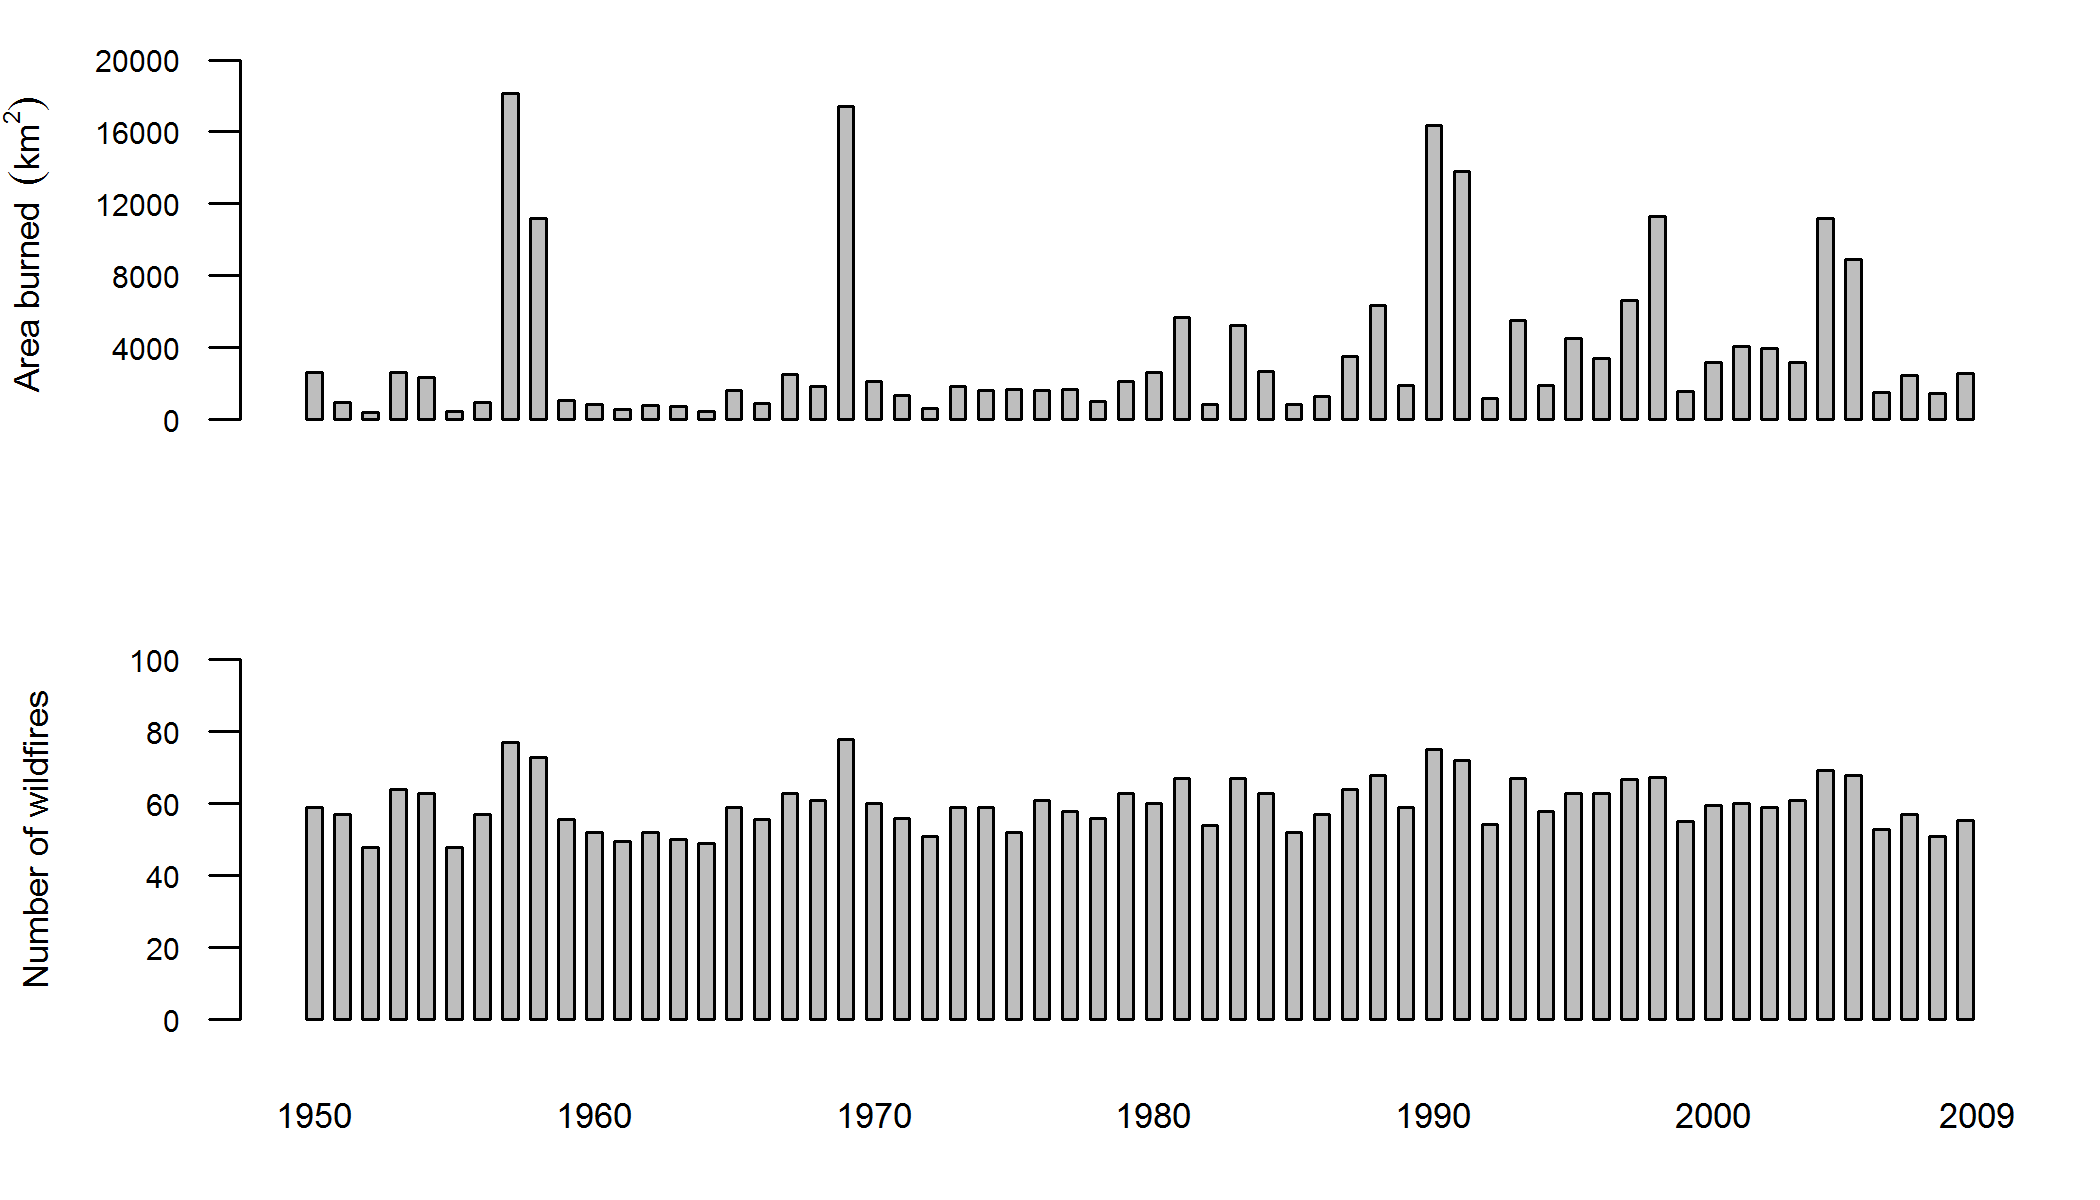
\includegraphics[width=\maxwidth]{figure/baseline_fire_barplot_AK-1} \caption[Alaska]{Alaska\label{fig:baseline_fire_barplot_AK}}
\end{figure}



\newpage
\subsection{LCC Regions}
All five following separate LCC graphs relate to figure 3.3 in the original document.
This uses strictly ALFRESCO output.
\begin{figure}[H]
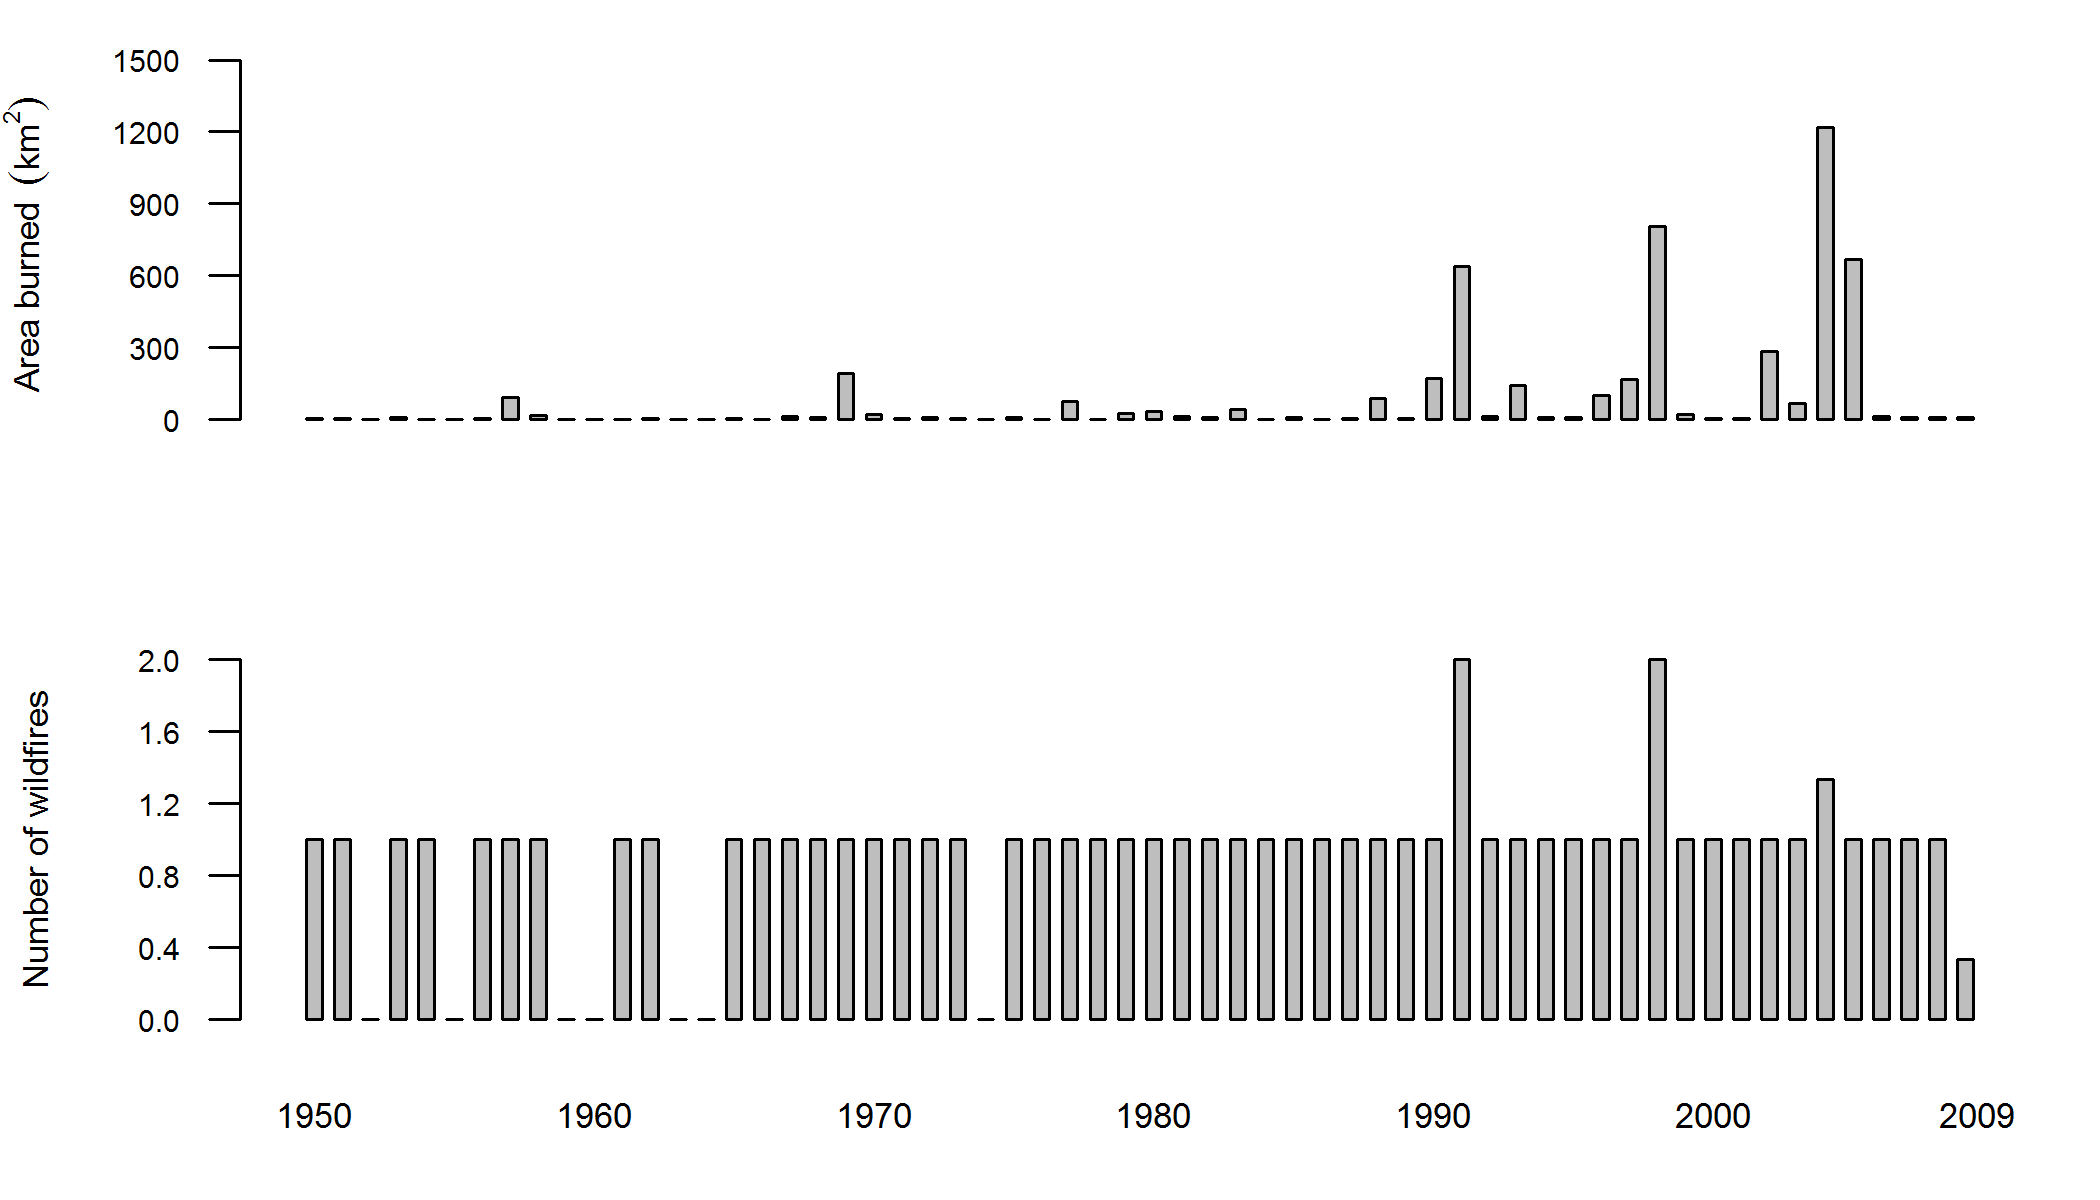
\includegraphics[width=\maxwidth]{figure/baseline_fire_barplot_LCC1-1} \caption[Arctic]{Arctic\label{fig:baseline_fire_barplot_LCC1}}
\end{figure}



\begin{figure}[H]
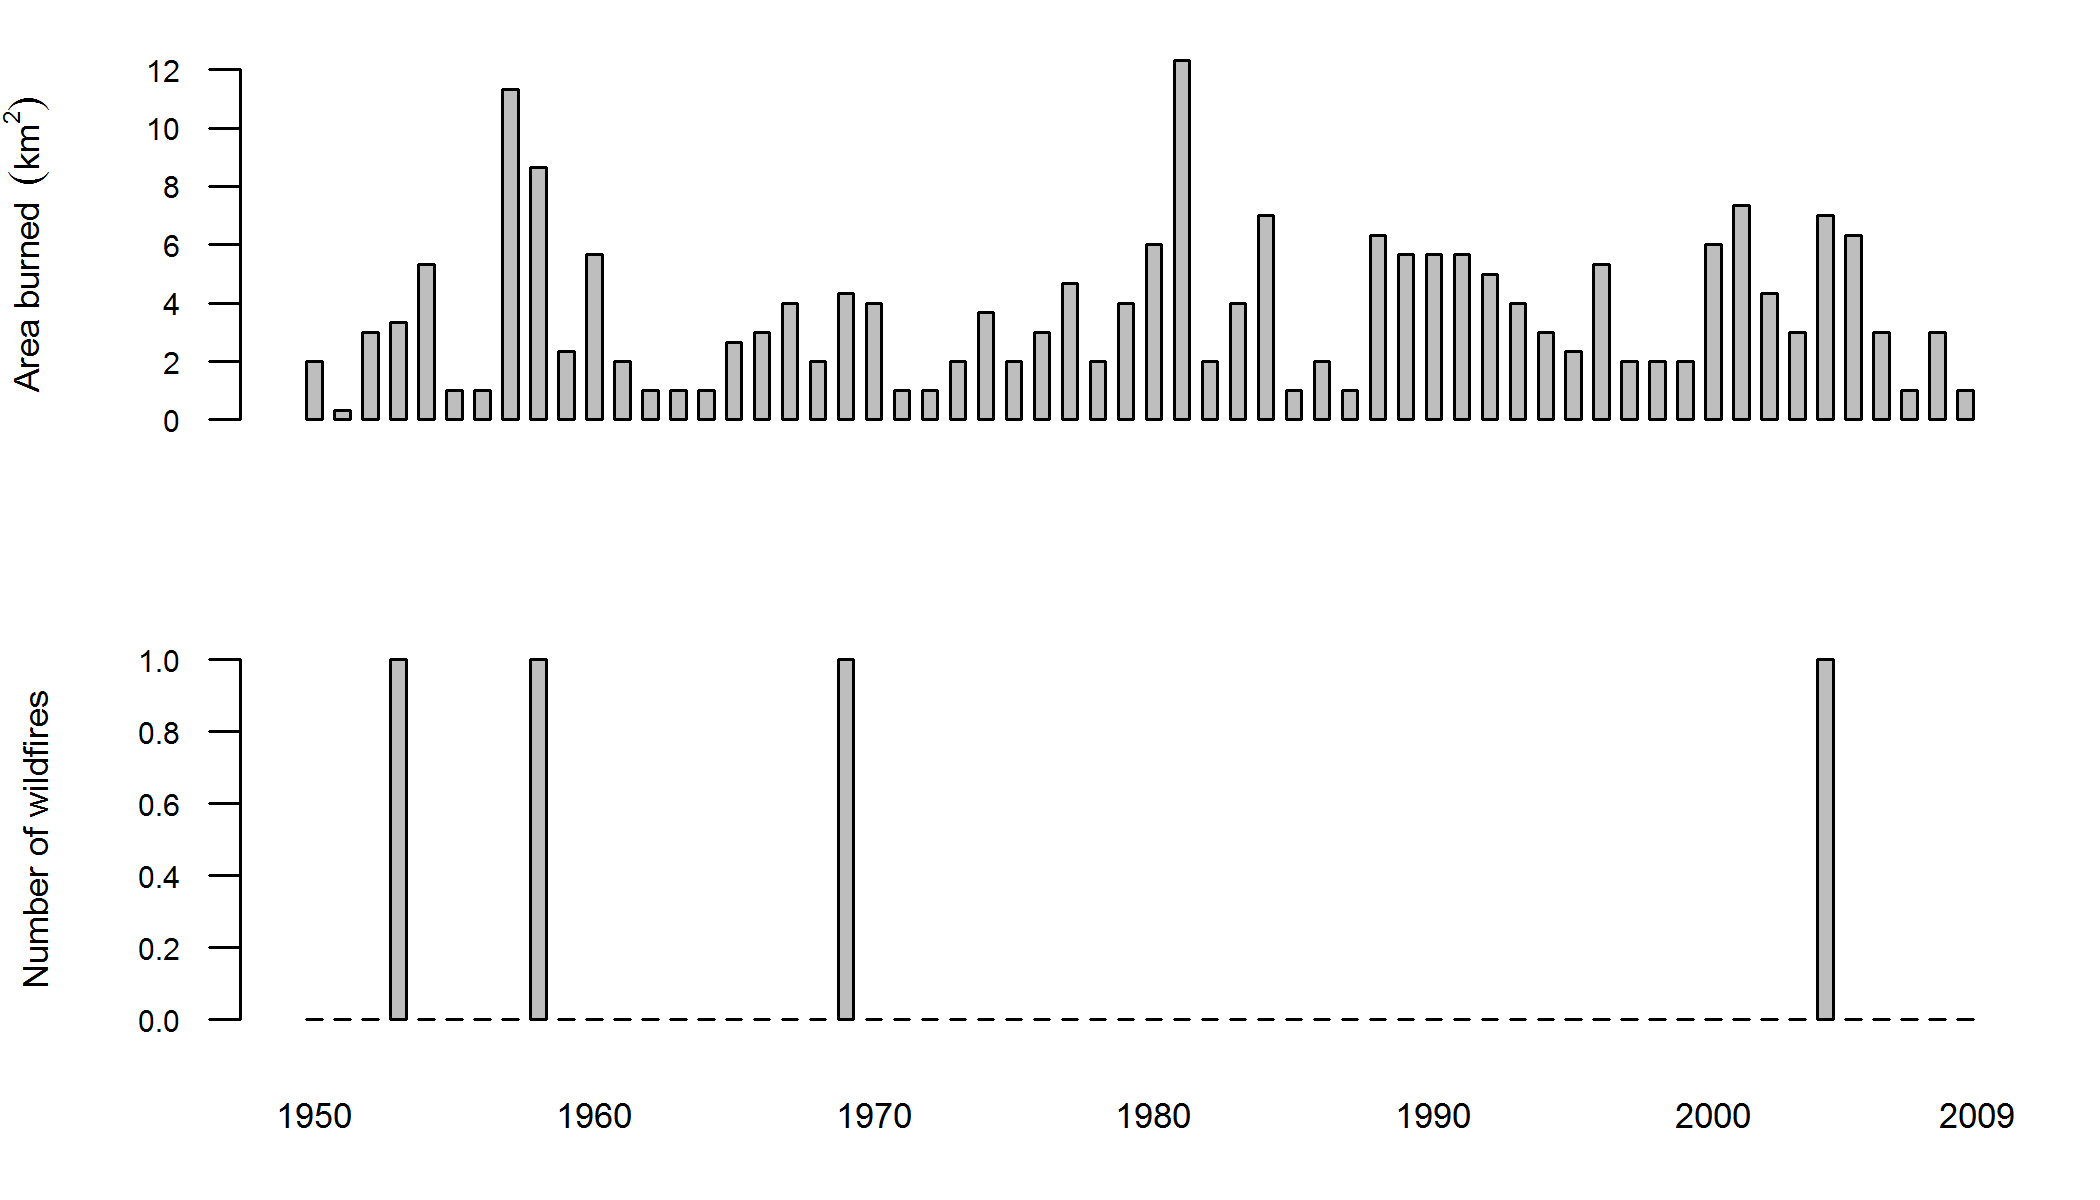
\includegraphics[width=\maxwidth]{figure/baseline_fire_barplot_LCC2-1} \caption[North Pacific]{North Pacific\label{fig:baseline_fire_barplot_LCC2}}
\end{figure}



\begin{figure}[H]
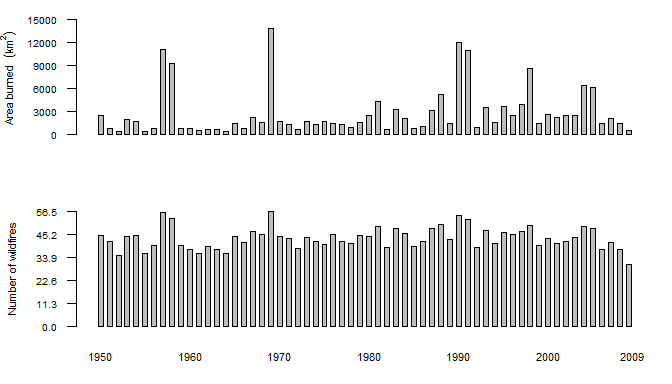
\includegraphics[width=\maxwidth]{figure/baseline_fire_barplot_LCC3-1} \caption[Northwest Interior Forest North]{Northwest Interior Forest North\label{fig:baseline_fire_barplot_LCC3}}
\end{figure}



\begin{figure}[H]
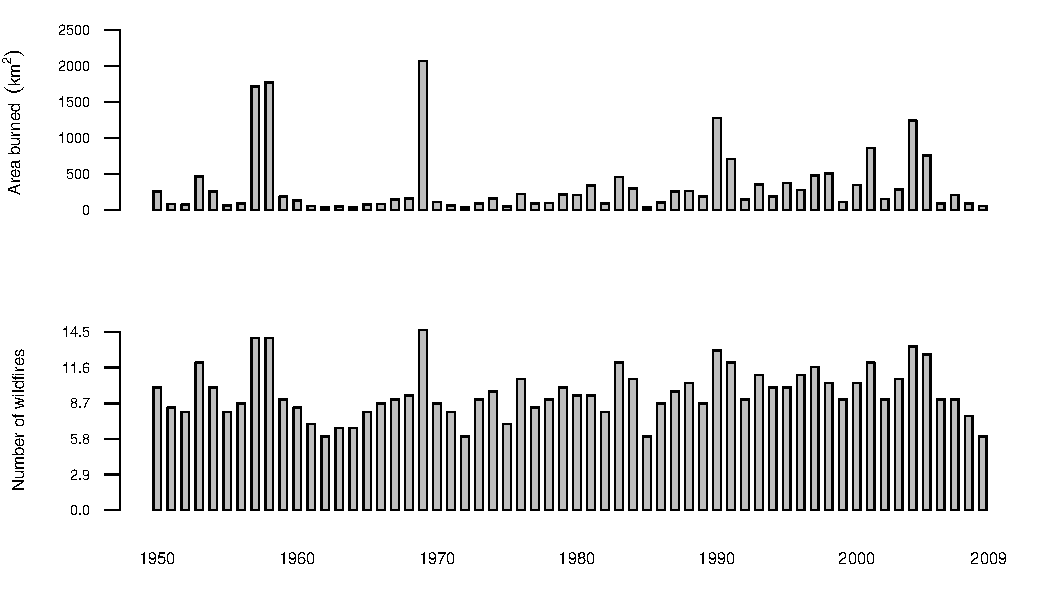
\includegraphics[width=\maxwidth]{figure/baseline_fire_barplot_LCC4-1} \caption[Northwest Interior Forest South]{Northwest Interior Forest South\label{fig:baseline_fire_barplot_LCC4}}
\end{figure}



\begin{figure}[H]
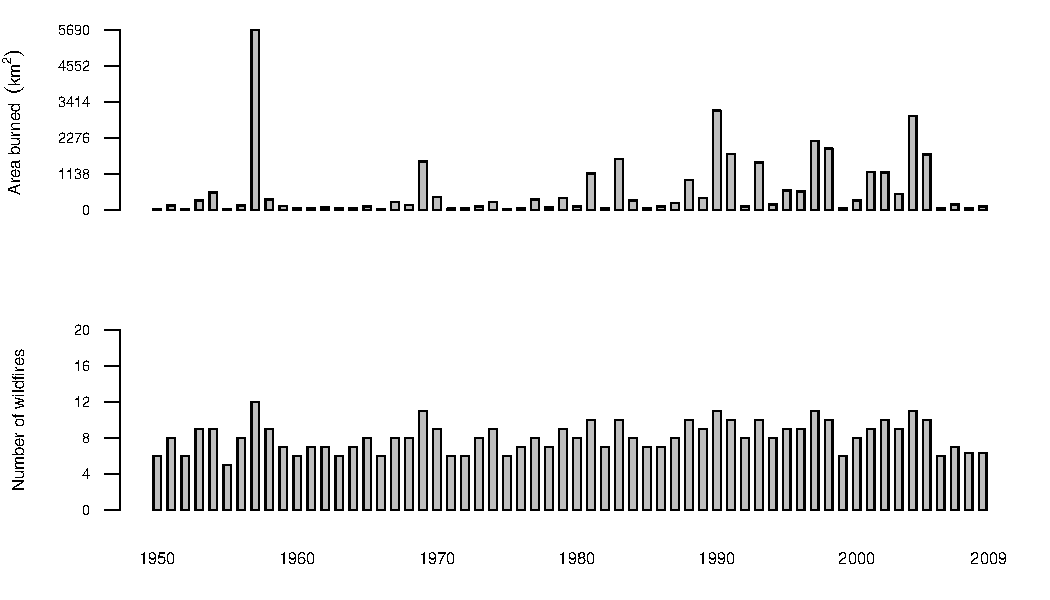
\includegraphics[width=\maxwidth]{figure/baseline_fire_barplot_LCC5-1} \caption[Western Alaska]{Western Alaska\label{fig:baseline_fire_barplot_LCC5}}
\end{figure}



\end{document}
